%Filename:   LG4.tex
%
\documentclass[12pt]{amsart}

%%%%%%%%%%%%%%%%%%%%%%%%%%%%%%%%%%%%%%%%%%%%%%%%%%%%%%%%%%%%%%%%%%%%%%%
%                              packages                               %
%%%%%%%%%%%%%%%%%%%%%%%%%%%%%%%%%%%%%%%%%%%%%%%%%%%%%%%%%%%%%%%%%%%%%%%
\usepackage{mathtools}
\usepackage{amsfonts,amsthm,amsmath,amssymb}
\usepackage{graphicx}
\usepackage[dvipsnames]{xcolor}
\usepackage{enumitem}
\usepackage{wrapfig}
\usepackage{ulem}  % rule out text

%%%%%%%%%%%%%%%  Layouts   Gives correct margins for 12 pt amsart  %%%%%%%%%%%%%% 
% 
%  US size paper 
% 
\headheight=8pt      \topmargin=0pt 
\textheight=613pt    \textwidth=466pt 
\oddsidemargin=1pt   \evensidemargin=1pt 

%%%%%%%%%%%%%%%%%%%%%%%%%%%%% Environments %%%%%%%%%%%%%%%%%%%%%%%%%%%%%%%%%%%%%%%%%%%%%%%%%%%%
\newtheorem{Theorem}{Theorem}[section]
\newtheorem{Proposition}[Theorem]{Proposition}
\newtheorem{Lemma}[Theorem]{Lemma}
\newtheorem{Corollary}[Theorem]{Corollary}
\newtheorem{Conjecture}[Theorem]{Conjecture}
\newtheorem{Fact}[Theorem]{Fact}

\theoremstyle{remark}
\newtheorem{Remark}[Theorem]{Remark}
\newtheorem{Example}[Theorem]{Example}
\newtheorem{Definition}[Theorem]{Definition}



%%%%%%%%%%%%%%%%%%%%%%%%%%%%%%%%%%%%%%%%%%%%%%%%%%%%%%%%%%%%%%%%%%%%%%%%%%%%%%%%%%%%%%%%%%%%%%%%%%%%
%                                Macros
\newcommand{\Gr}{\textit{Gr\,}}
\newcommand{\Hom}{\textrm{Hom}}
\newcommand{\LG}{\textit{LG}}
\newcommand{\pr}{\textit{pr}}
\newcommand{\Span}{\textrm{span}}

\newcommand{\CC}{{\mathbb C}}
\newcommand{\PP}{{\mathbb P}}
\newcommand{\ZZ}{{\mathbb Z}}

\newcommand{\ndot}{\mbox{{\tiny$\bullet$}}}

%
% Tableaux
%
\newcommand{\I}{
\includegraphics{images/1.eps}}
\newcommand{\TI}{
\includegraphics{images/21.eps}}
\newcommand{\ThI}{
\includegraphics{images/31.eps}}
\newcommand{\Th}{
\includegraphics{images/3.eps}}

\newcommand{\sI}{
\includegraphics{images/s1.eps}}
\newcommand{\sTI}{
\includegraphics{images/s21.eps}}
\newcommand{\sThI}{
\includegraphics{images/s31.eps}}
\newcommand{\sTh}{
\includegraphics{images/s3.eps}}

\newcommand{\schTI}{\raisebox{-2pt}{\sTI\hspace{.5pt}}}
\newcommand{\schThI}{\raisebox{-2pt}{\sThI\hspace{.5pt}}}

\newcommand{\tTT}{
\includegraphics{images/t22.eps}}
\newcommand{\tTIc}{
\includegraphics{images/t21c.eps}}

\newcommand{\defcolor}[1]{{\color{blue}#1}}
\newcommand{\demph}[1]{\defcolor{{\sl #1}}}


%%%%%%%%%%%%%%%%%%%%%%%%%%%%%%%%%%%%%%%%%%%%%%%%%%%%%%%%%%%%%%%%%%%%%%%%%%%%%%%%%%%%%%%%%%%%%%%%%%%%
\title{Enriched Schubert problems in the Grassmannian  \\ of Lagrangian subspaces in 8-space}
%%%%%%%%%%%%%%%%%%%%%%%%%%%%%%%%%%%%%%%%%%%%%%%%%%%%%%%%%%%%%%%%%%%%%%%%%%%%%%%%%%%%%%%%%%%%%%%%%%%%
\author{F.~Sottile}
\address{Frank Sottile, Department of Mathematics,
         Texas A\&M University, College Station, Texas 77843,  USA}
\email{sottile@math.tamu.edu}
\urladdr{http://www.math.tamu.edu/\~{}sottile}
%%%%%%%%%%%%%%%%%%%%%%%%%%%%%%%%%%%%%%%%%%%%%%%%%%%%%%%%%%%%%%%%%%%%%%%%%%%%%%%%%%%%%%%%%%%%%%%%%%%%
\thanks{Research of Sottile supported in part by NSF grant  DMS-2201005.}
%%%%%%%%%%%%%%%%%%%%%%%%%%%%%%%%%%%%%%%%%%%%%%%%%%%%%%%%%%%%%%%%%%%%%%%%%%%%%%%%%%%%%%%%%%%%%%%%%%%%
\subjclass{}
%
%
%
\keywords{Lagrangian Grassmannian, Galois groups, Schubert problem}
%%%%%%%%%%%%%%%%%%%%%%%%%%%%%%%%%%%%%%%%%%%%%%%%%%%%%%%%%%%%%%%%%%%%%%%%%%%%%%%%%%%%%%%%%%%%%%%%%%%%


%%%%%%%%%%%%%%%%%%%%%%%%%%%%%%%%%%%%%%%%%%%%%%%%%%%%%%%%%%%%%%%%%%%%%%%%%%%%%%%%%%%%%%%%%%%%%%%%%%%%
\begin{document}

%%%%%%%%%%%%%%%%%%%%%%%%%%%%%%%%%%%%%%%%%%%%%%%%%%%%%%%%%%%%%%%%%%%%%%%%%%%%%%%%%%%%%%%%%%%%%%%%%%%%
\begin{abstract}
  We describe the three enriched Schubert problems on the Lagrangian Grassmannian $\LG(4)$ of isotropic 4-planes in 8-space,
  and use that to determine their Galois groups. (This is in progress.)
\end{abstract}
%%%%%%%%%%%%%%%%%%%%%%%%%%%%%%%%%%%%%%%%%%%%%%%%%%%%%%%%%%%%%%%%%%%%%%%%%%%%%%%%%%%%%%%%%%%%%%%%%%%%
\maketitle


\section{Preliminary calculations}
Using the Frobenius algorithm, we determined that three of the 44 essential Schubert problems on $\LG(4)$ are enriched.
For one, with 384 solutions, we are still computing Frobenius elements.
We have yet to be able to compute an eliminant for a problem with 768 solutions.

Using strict partitions to represent Schubert conditions, these three problems are
\[
  \raisebox{-8pt}{\TI\,}^2\cdot\, \raisebox{-8pt}{\ThI}\ =\ 4\,, \quad
  \raisebox{-8pt}{\TI\,}^2\cdot\, \raisebox{-2pt}{\Th}\cdot\, \raisebox{-2pt}{\I}\ =\ 4\,, \quad\mbox{ and } \quad
  \raisebox{-8pt}{\TI\,}^3\cdot\, \raisebox{-2pt}{\I}\ =\ 8\,.
\]


Let $V\simeq\CC^8$ be a vector space equipped with a nondegenerate alternating form \defcolor{$\langle\ndot,\ndot\rangle$}.
We call $(V,\langle\ndot,\ndot\rangle)$ a \demph{symplectic vector space}.
The annihilator of a linear space $H$ of $V$ is $ \defcolor{H^{\angle}}:= \{v\in V\mid \langle u,v\rangle = 0\ \forall u\in H\}$.
As $\langle\ndot,\ndot\rangle$ is nondegenerate, $\dim H + \dim H^\angle=\dim V$.
A subspace $H\subset V$ is \demph{isotropic} if $H\subset H^{\angle}$.
Then the dimension of an isotropic subspace $H$ is at most $\frac{1}{2}\dim V$, and it is  \demph{Lagrangian} (maximal isotropic) if
$\dim H = \frac{1}{2}\dim V$.
Write \defcolor{$\LG(V)$} or \defcolor{$\LG(4)$} for the space of Lagrangian subspaces of $V$.
This is a ten-dimensional smooth subvariety of \defcolor{$\Gr(4,V)$}, the Grassmannian of 4-planes in $V$.
We will assume that the reader is familiar with our terminology, as well as the basics of Schubert calculus on $\LG(V)$.

Let $L,M\in\LG(V)$ be two general Lagrangian subspaces.
In particular $L\cap M=\{0\}$ so that the map $L\oplus M\to V$ defined by $u\oplus v\mapsto u+v$ is an isomorphism.
For $0\neq v\in M$ consider the linear function $\Lambda_v\colon L\to \CC$ defined by $\Lambda_v(u)=\langle u,v\rangle$.
As $L$ is Lagrangian and $L\cap M=\{0\}$, this linear form is nonzero on $L$.
In particular, $v\mapsto \Lambda_v$ identifies $M$ with the linear dual $\defcolor{L^*}:=\Hom(L,\CC)$ of $L$.

Suppose that $N\in\LG(V)$ is a third Lagrangian subspace in general position with respect to both $L$ and $M$.
Then the projections  \defcolor{$\pi_L$} and \defcolor{$\pi_M$} of $N$ to the summands in $L\oplus M\simeq V$ are isomorphisms.
This identifies $N$ as the graph of a linear isomorphism
\[
\defcolor{\varphi_N}\ :=\ \pi_M\circ\pi_L^{-1}\ \colon\ L\ \xrightarrow{\ \sim\ }\  M\,.
\]
This linear isomorphism $\varphi_N\colon L\to M\simeq L^*$  induces a nondegenerate bilinear form \defcolor{$(\ndot,\ndot)_N$} on $L$ which
is defined for $u,u\in L$ by $(u,u')_N:=\langle u, \varphi_N(u')\rangle$.

The bilinear form $(\ndot,\ndot)_N$ is symmetric.
Indeed, as $N$ is isotropic, we have that for $u,u'\in L$, $u+\varphi_N(u)$ and $u'+\varphi_N(u')$ lie in $N$ so that
%
 \begin{multline*}
   \qquad 0\ =\  \langle u+\varphi_N(u)\,,\, u'+\varphi_N(u')\rangle
   \\
    \ =\
    \langle u\,,\,u' \rangle \ +\ 
    \langle u\,,\,\varphi_N(u') \rangle  \ +\ 
    \langle \varphi_N(u)\,,\,u' \rangle \ +\ 
    \langle \varphi_N(u)\,,\,\varphi_N(u') \rangle\,. \qquad
 \end{multline*}
%
As $u,u'\in L$ and $\varphi_N(u),\varphi_N(u')\in M$, we see that $0 = \langle u,\varphi_N(u') \rangle   + \langle \varphi_N(u),u' \rangle$, 
so that $\langle u,\varphi_N(u') \rangle =\langle u',\varphi_N(u) \rangle$, as $\langle\ndot,\ndot\rangle$ is alternating.
Thus $(u,u')_N=(u',u)_N$  is symmetric.


Define $\defcolor{\schTI(L)}:=\{H\in\LG(V)\mid \dim H\cap L\geq 2\}$, which is a Schubert subvariety of codimension three in $\LG(V)$.
It is the intersection of $\LG(V)$ with the Schubert subvariety $\Omega_{\tTT}(L)$  of the Grassmannian $\Gr(4,V)$.
Set $\defcolor{X(L,M)}:=\schTI(L)\cap\schTI(M)$, a Richardson variety.
If $H\in X(L,M)$, then $H\cap L\in\Gr(2,L)$ and  $H\cap M\in\Gr(2,M)$.
If we set $\defcolor{h}:=H\cap L$ and $h':=H\cap M$, then $H=h\oplus h'$.
As $H$ is isotropic, $\langle h,h'\rangle\equiv 0$, which implies that $h'$ is the annihilator \defcolor{$h^\perp$} of $h$ in $M=L^*$.

Following work on the Pieri formula in isotropic Schubert calculus~\cite{MaxPieri} (see also~\cite{EPieri}), 
it is useful to define the union, $Z(L,M)$, of the linear spaces in $X(L,M)$,
\[
\defcolor{Z(L,M)}\ :=\  \bigcup\{ H\ \mid\ H\in X(L,M)\}\,,
\]
which we  consider to be a subvariety of the projective space $\PP(V)$.
More formally and working projectively, let
\[
\defcolor{C(1,4;V)}\ :=\ \{(\ell,H)\mid H\in\LG(V)\mbox{ and }\ell\in\PP(H)\}
\]
be the symplectic flag variety of
isotropic lines lying on Lagrangian subspaces in $V$.
This has projections to projective space $\PP(V)$ and to the Lagrangian Grsassmannian.
%
\[
  \begin{picture}(122,55)
    \put(33,46){$C(1,4;V)$}
    \put(50,42){\vector(-1,-1){30}}      \put(72,42){\vector(1,-1){30}}
    \put(24,27){\small$\pr$}           \put(89,27){\small$\pi$}
    \put(0,0){$\PP(V)$}   \put(88,0){$\LG(V)$}
  \end{picture}
\]
%
Each realizes $C(1,4;V)$ as a fibre bundle, with $\pi^{-1}(H)=\PP(H)\simeq\PP^3$ and $\pr^{-1}(\ell)=\LG(3,\ell^\angle/\ell)$.
Then $Z(L,M):=\pr\circ\pi^{-1}(X(L,M))$.
Define
\[
\defcolor{Y(L,M)}\ :=\ \pi^{-1}(X(L,M))\subset C(1,4;V)\,.
\]

For $0\neq u\in L$, let $u^\perp \subset M$ be its annihilator, which is 3-dimensional.
Similarly, for $0\neq v\in M$, let $v^\perp\subset L$ be its annihilator.


%%%%%%%%%%%%%%%%%%%%%%%%%%%%%%%%%%%%%%%%%%%%%%%%%%%%%%%%%%%%%%%%%%%%%%%%%%%%%%%%%%%%%%%%%%%%%%%%%%%%
\begin{Lemma}
  \label{L:quadrics}
  In the coordinates $\{(u,v)\mid u\in L\mbox{ and }v\in M\}$ for $\PP(V)$, the variety $Z(L,M)$ is the quadratic hypersurface with 
  equation $\langle u,v\rangle = 0$.
  The map $\pr\colon Y(L,M)\to Z(L,M)$ has fibre over a point $(u,v)\in Z(L,M)$ identified with $\PP(v^\perp/u)$.
  When $u$ and $v$ are nonzero, this is isomorphic to $\PP^1$; otherwise it is isomorphic to $\PP^2$.
  
  Let $(u,v)\in Z(L,M)$ with $u$ and $v$ both nonzero.
  If we restrict the maps $\pi,\pr$ to $Y(L,M)$, then the set
%
  \begin{equation}
  \label{Eq:quadric}
     \bigcup\{ H\in X(L,M)\mid (u,v)\in H\}\ =\ \pr \circ \pi^{-1} \circ \pi \circ \pr^{-1}(u,v)\,,
  \end{equation}
%
  is the quadric hypersurface $Z(L,M,u,v):=Z(L,M)\cap \PP(v^\perp\oplus u^\perp)$ in $\PP(v^\perp\oplus u^\perp)\simeq\PP^5$, and the map
  between $\pi \circ \pr^{-1}(u,v) \subset\LG(V)$ and $Z(L,M,u,v)$ is birational away from the exceptional divisor
  $\PP(u + v^\perp) \cup \PP(u^\perp+v)$.
\end{Lemma}
%%%%%%%%%%%%%%%%%%%%%%%%%%%%%%%%%%%%%%%%%%%%%%%%%%%%%%%%%%%%%%%%%%%%%%%%%%%%%%%%%%%%%%%%%%%%%%%%%%%%
\begin{proof}
  A Lagrangian subspace $H\in X(L,M)$ has the form $h\oplus h^\perp$ for $h\in\Gr(2,L)$.
  Thus if $(u,v)\in H$, then $u\in h$ and $v\in h^\perp$, so that $\langle u,v\rangle=0$,
  and we have that $u\in h\subset v^\perp$.
  A point $(u,v)\in V$ with  $\langle u,v\rangle=0$ has $u\in v^\perp \subset L$.
  Given any $h\in\Gr(2,L)$ with $u\in H\subset v^\perp$, we have $v\in h^\perp$ so that
  $(u,v)\in h\oplus h^\perp \in X(L,M)$.
  This shows that $Z(L,M)$ equals the quadratic hypersurface and that the fibre $\pr^{-1}(u,v)=\PP(v^\perp/u)$.
  Since at most one of $u$ or $v$ may be zero, this is ispmorphic to $\PP^2$ if one is zero and $\PP^1$ if neither is zero.

  For the last statement, note that the set~\eqref{Eq:quadric} is contained in $Z(L,M)\cap \PP(v^\perp\oplus u^\perp)$.
  Indeed, suppose that $(u,v)\in H$ and $H\in X(L,M)$.
  Then $H=h\oplus h^\perp$ and $u\in h\subset v^\perp$ and $v\in h^\perp\subset u^\perp$.
  If $(a,b)\in H$, then $a\in v^\perp$ and $b\in u^\perp$, and $\langle a,b\rangle = 0$.
  
  Let $(a,b)\in Z(L,M)\cap \PP(v^\perp\oplus u^\perp)$.
  Suppose that $a$ is linearly independent of $u$ and $b$ is linearly indepedent of $v$.
  As $u,a\in L$, $v,b\in M$, $a\in v^\perp$ and $b\in u^\perp$,
  $\Span\{a,u\}$ annihilates $\Span\{b,v\}$, so that $\Span\{a,b,u,v\}$ is the unique Lagrangian subspace containing these four 
  points. 
\end{proof}
%%%%%%%%%%%%%%%%%%%%%%%%%%%%%%%%%%%%%%%%%%%%%%%%%%%%%%%%%%%%%%%%%%%%%%%%%%%%%%%%%%%%%%%%%%%%%%%%%%%%

{\color{Magenta}The quadric $Z(L,M,u,v)$ is singular; it is the cone over a quadric isomorphic to $\PP(v^\perp/u)\times\PP(u^\perp/v)$ in a
  $\PP^3$ with vertex $\PP(u+v)$, a $\PP^1$.} 


%%%%%%%%%%%%%%%%%%%%%%%%%%%%%%%%%%%%%%%%%%%%%%%%%%%%%%%%%%%%%%%%%%%%%%%%%%%%%%%%%%%%%%%%%%%%%%%%%%%%
\subsection{The Galois group of $\schTI^2\cdot\sTh\cdot\sI=4$ is $D_4$.}

Let $L$, $M$, and $N$ be general Lagrangian subspaces in $V$ as before, and let $m$ be an isotropic 2-plane, also in general position.
Observe that 
%
 \begin{equation}
  \label{Eq:intersection} 
     \schTI(L)\cap\schTI(M)\cap \sTh(m)\ =\ \pi \bigl( \pr^{-1}(m\cap Z(L,M))\bigr)\,.
 \end{equation}
%
By Lemma~\ref{L:quadrics}, $Z(L,M)$ is a quadric.
Thus it meets $m$ in two points $(u,v)$ and $(u',v')$, showing that the intersection~\eqref{Eq:intersection}  has two components.

Let $W$ be the component of~\eqref{Eq:intersection} coming from $(u,v)$.
By Lemma~\ref{L:quadrics} again, if we restrict $\pi$ to $Y(L,M)$, then  $\pr(\pi^{-1}(W))=Z(L,M)\cap\PP(u^\perp\oplus v^\perp)=Z(L,M,u,v)$
is a quadric hypersurface in the $\PP^5\simeq \PP(u^\perp\oplus v^\perp)$.
Each of the two points of intersection of $N$ with $Z(L,M,u,v)$ gives a solution to the Schubert problem
%
 \begin{equation}
   \label{Eq:TIe2Th.I=4}
   \schTI(L)\cap\schTI(M)\cap \sTh(m)\cap \sI(N)\,.
 \end{equation}
%
With the other point $(u',v')$ of $m\cap Z(L,M)$, this gives four solutions to the Schubert problem~\eqref{Eq:TIe2Th.I=4}.
Note that $N$ is spanned by its intersections with  $Z(L,M,u,v)$  and  $Z(L,M,u',v')$ 
As its Galois group must preserve the partition coming from the two points $(u,v)$ and $(u',v')$, it is a subgroup of $D_4$.
We have computed Frobenius elements which show that the Galois group is $D_4$.

For an alternative proof, note that it is possible to find a the monodromy loop that fixes $L,M,m$ (and hence the points $(u,v)$ and
$(u',v')$), as well as the two points $N\cap Z(L,M,u,v)$, but interchanges the other two points  $N\cap Z(L,M,u',v')$.
Indeed, let $\{x,y\}=N\cap Z(L,M,u,v)$.
Then the set of Lagrangian planes containing $h := \Span{x,y}$ is identified with $\LG(h^\angle/h)$, and any two points in
$\PP(x^\angle)\cap\PP(y^\angle)$ that are independent.
{\color{Magenta}Fix this.  It is important to make these kinds of arguments.}



%choosing a path $\gamma\subset Z(L,M,u',v')^2$ that interchanges the other two points $N\cap Z(L,M,u',v')$, we see that the
%
%
%We must argue that this gives a valid monodromy loop in that it is possible to choose the path $\gamma$ so that the span of
%$N\cap Z(L,M,u,v)$ and the pairs of points in $\gamma$ is always a Lagrangian subspace.
%
% using a path in $Z(L,M,u',v')\cap \PP(u^\perp\oplus v^\perp)$ (to ensure that the
%family of $are allowed to vary, 
%\footnote{need to make this more precise.}


%%%%%%%%%%%%%%%%%%%%%%%%%%%%%%%%%%%%%%%%%%%%%%%%%%%%%%%%%%%%%%%%%%%%%%%%%%%%%%%%%%%%%%%%%%%%%%%%%%%%
\subsection{The Galois group of $\schTI^2\cdot\schThI=4$ is $\ZZ_2\times\ZZ_2$.}

Let $L,M,N$ be as before, and consider a Lagrangian subspace $H\in\schTI(L)\cap\schTI(M)\cap\schTI(N)$.
As $H\in\schTI(L)\cap\schTI(M)$, it has the form $h\oplus h^\perp$ for $h\in\Gr(2,L)$, and it is not hard to see that $h^\perp=\varphi_N(h)$.
These together imply that $(h,h)_N\equiv 0$, so that $h$ is an isotropic 2-plane in the linear space $L\simeq\CC^4$ equipped with the
nondegenerate symmetric form $(\ndot,\ndot)_N$.
Let us work in $\PP(L)$.
Then $h$ lies in one of the two families of lines that rule the quadric surface $\defcolor{Q_N}\vcentcolon=\{u\in\PP(L)\mid (u,u)_N=0\}$
in $\PP(L)$.
Now let $\ell\subset L$ be an isotropic 2-plane in $L$, which is a line in $\PP(L)$.
This will meet $Q$ in two points, and through each point there will be two lines---one in each ruling.
These four solutions $h$ give the four solutions $h\oplus h^\perp$ to the Schubert problem.

The partition of the four solutions by the corresponding points of intersection $\ell\cap Q$ show that the Galois group is a subgroup of
$D_4$.
To analyze this further, let $p$ and $q$ be the two points in $\ell\cap Q_N$, and let the four lines on $Q_N$ meeting these points be
$h^1_p$, $h^2_p$, $h^1_q$, and $h^2_q$, with the upper index representing the ruling of $Q_N$ the line lies in and the lower indicating the
point of $\ell\cap Q_N$ it meets.
However,  there are two solution lines $h$ in each ruling and the Galois group must preserve their intersections.
Consequently, the Galois group is the Klein 4-group, isomorphic to  $\ZZ_2\times\ZZ_2$.
\[
\fbox{\begin{picture}(200,120)
    \put(0,0){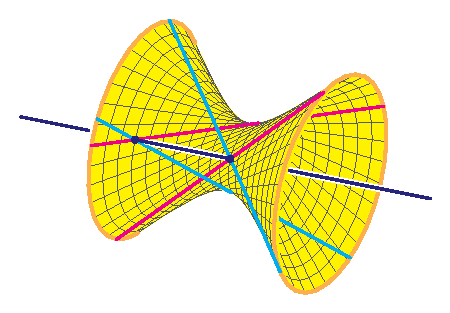
\includegraphics[height=120pt]{images/TIe2ThI.4.eps}}
    \put(4,65){$\ell$}
    \put(30,95){$Q_N$}
    
   \end{picture}}
\]

%%%%%%%%%%%%%%%%%%%%%%%%%%%%%%%%%%%%%%%%%%%%%%%%%%%%%%%%%%%%%%%%%%%%%%%%%%%%%%%%%%%%%%%%%%%%%%%%%%%%
\subsection{The Galois group of $\schTI^3\cdot\sI=8$  is not yet determined.}







%%%%%%%%%%%%%%%%%%%%%%%%%%%%%%%%%%%%%%%%%%%%%%%%%%%%%%%%%%%%%%%%%%%%%%%%%%%%%%%%%%%%%%%%%%%%%%%%%%%%
\bibliographystyle{amsplain}
\bibliography{LG4.bib}
%%%%%%%%%%%%%%%%%%%%%%%%%%%%%%%%%%%%%%%%%%%%%%%%%%%%%%%%%%%%%%%%%%%%%%%%%%%%%%%%%%%%%%%%%%%%%%%%%%%%

\end{document}
